% --------------------------------------------------
% 
% This chapter is for PEMA and DARN 
% 
% --------------------------------------------------

\chapter{Software development to establish quality HTS-oriented bioinformatics methods for microbial diversity assessment}
\label{cha:2}


% SECTION 1
\section{Environmental DNA metabarcoding: challenges and caveats}

% Building up a flexible and scalable pipeline for environmental DNA Metabarcoding Analysis

\newpage

% SECTION 2
\section{PEMA: a flexible Pipeline for Environmental DNA Metabarcoding Analysis of the 16S/18S ribosomal RNA, ITS, and COI marker genes}


Publication relative to this chapter: \cite{zafeiropoulos2020pema}. 


\begin{figure}[!htbp]
   \centering
   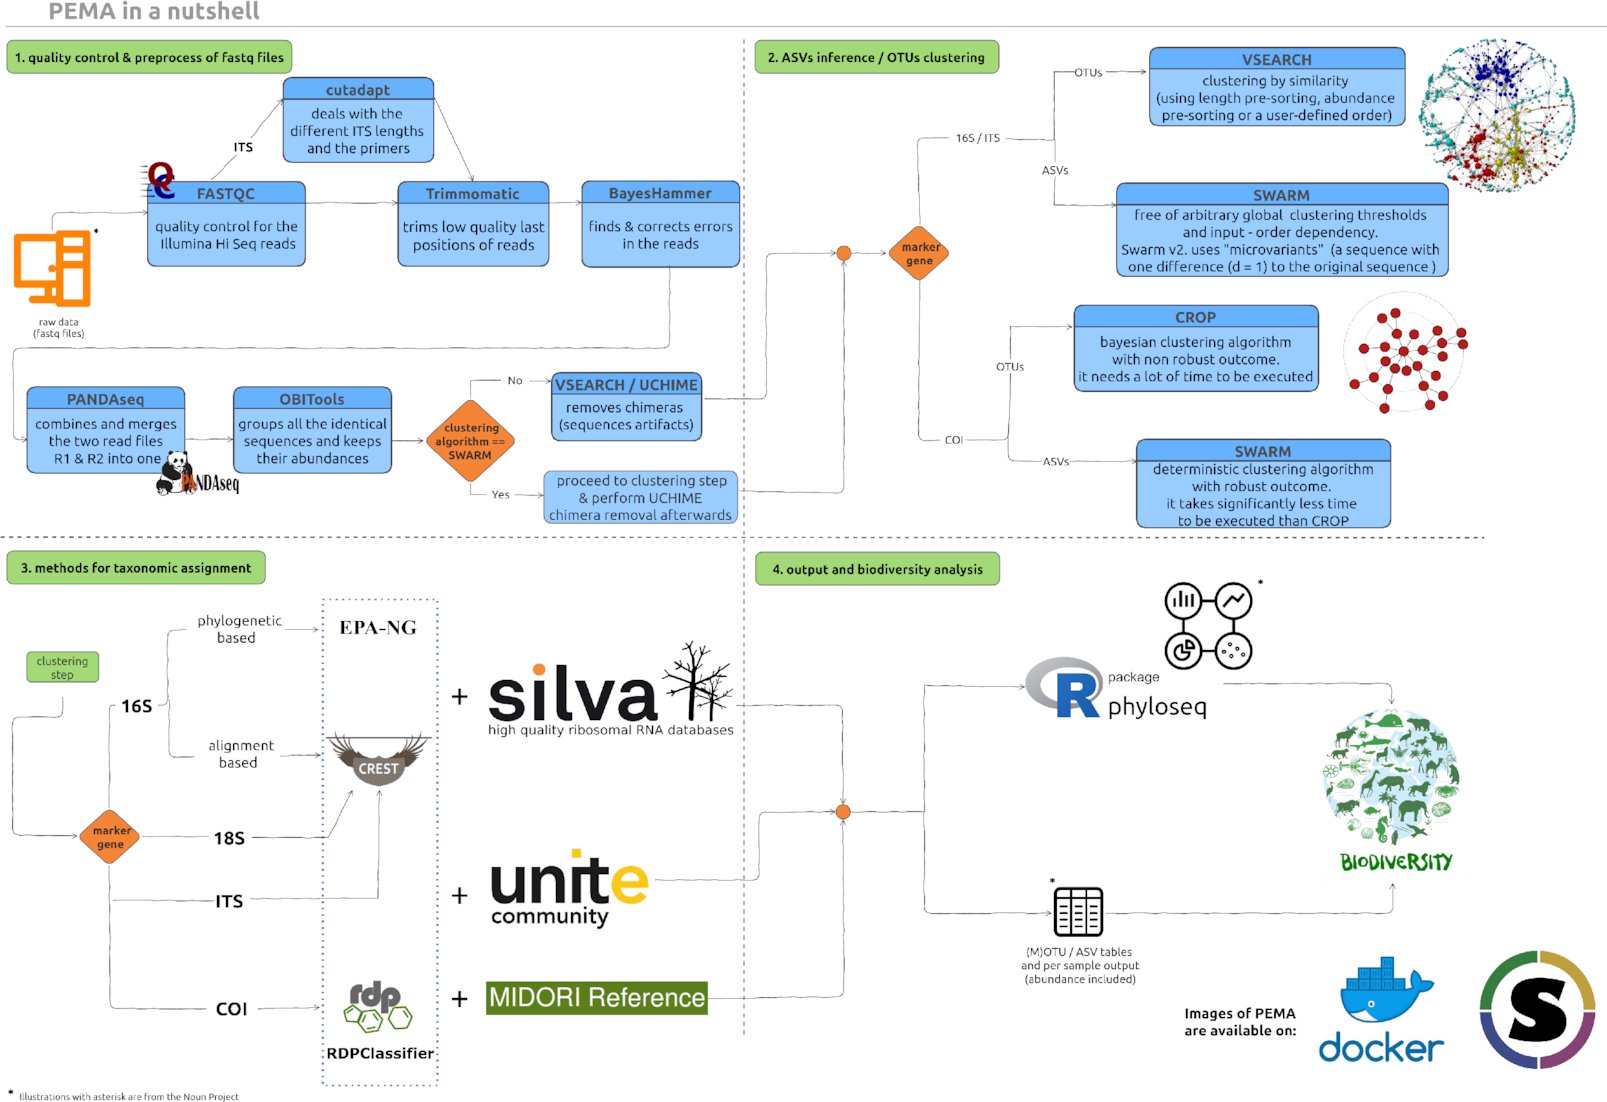
\includegraphics[width=0.95\columnwidth]{figures/pema_workflow.jpeg}
   \caption{The PEMA workflow: figure from publication}
\end{figure}



\newpage

% SECTION 3
\section{The Dark mAtteR iNvestigator (DARN) tool: getting to know the known unknowns in COI amplicon data}

Publication relative to this chapter: \citep{zafeiropoulos2021dark}


\begin{figure}[!htbp]
   \centering
   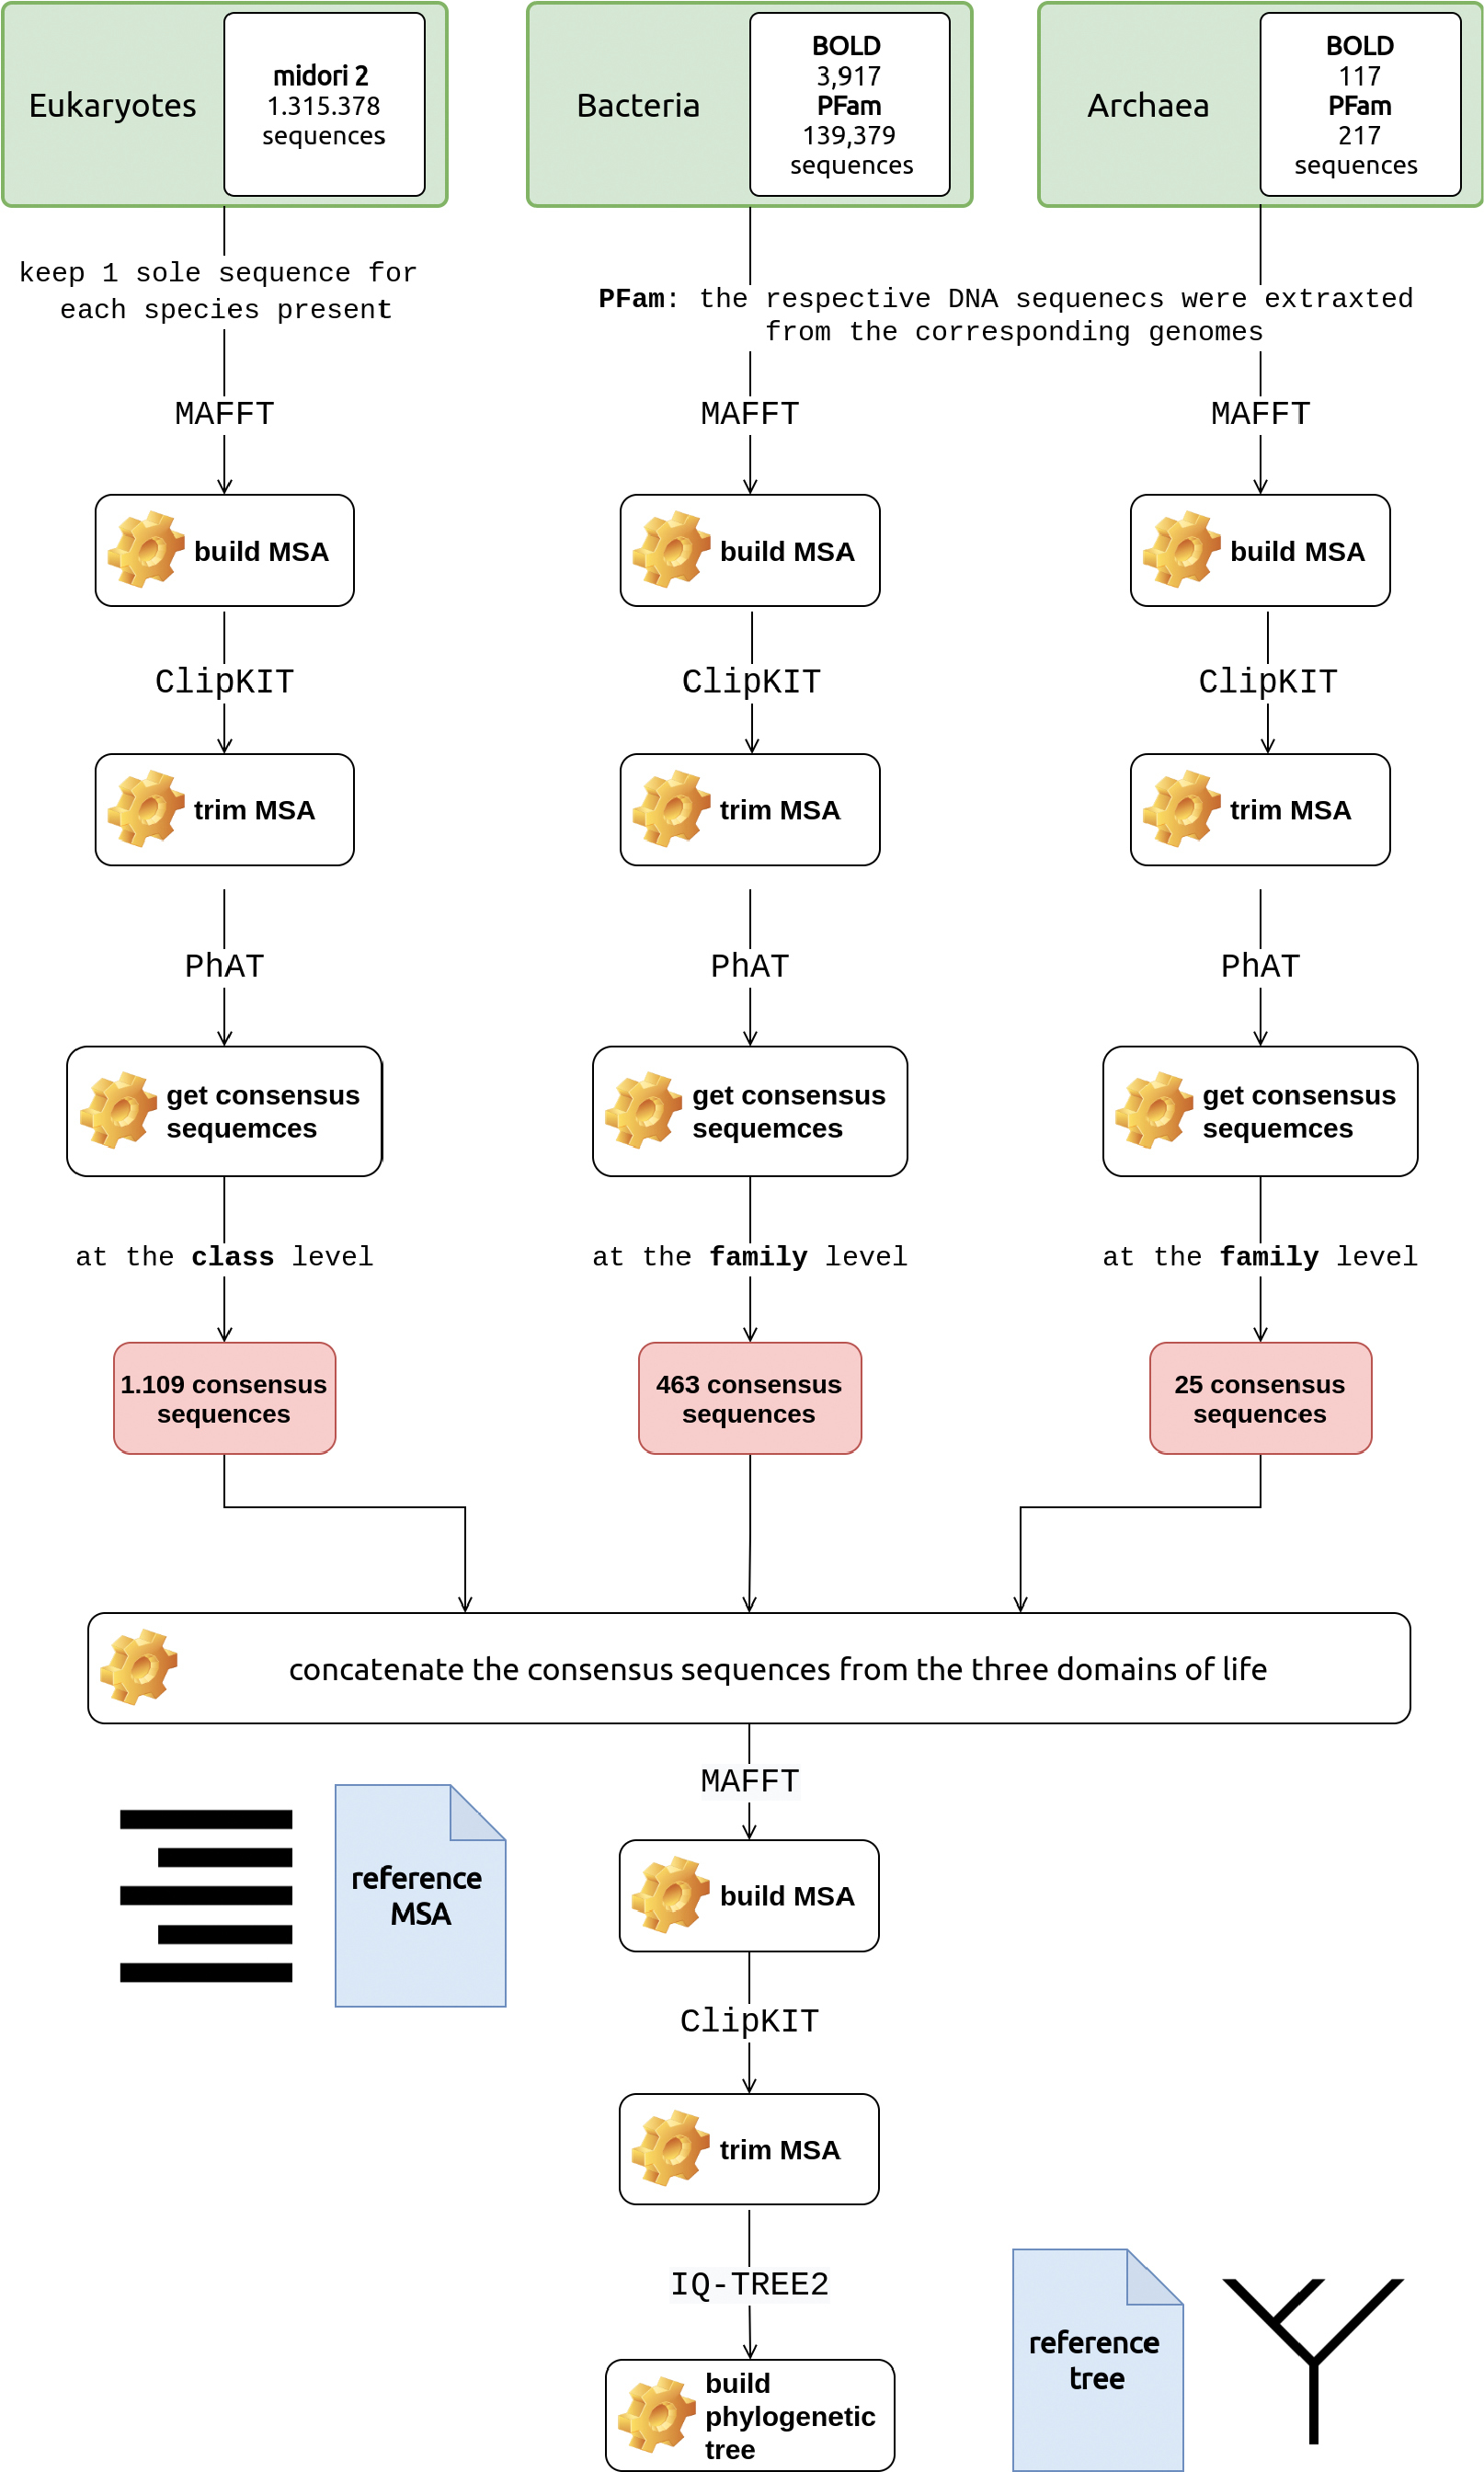
\includegraphics[width=0.75\columnwidth]{figures/darn_methodology.jpg}
   \caption{DARN methodology: figure in the publication}
\end{figure}

% % Table with COI and COI like sequences per rersource per domain
% \begin{table}[!htbp]
%    \begin{tabular}{lllll}
%    \hline
%    \multicolumn{1}{|l|}{\multirow{2}{*}{Resources}} & \multicolumn{2}{l|}{bacteria}                                             & \multicolumn{2}{l|}{archaea}                                              \\ \cline{2-5} 
%    \multicolumn{1}{|l|}{}                           & \multicolumn{1}{l|}{\# of sequences} & \multicolumn{1}{l|}{\# of strains} & \multicolumn{1}{l|}{\# of sequences} & \multicolumn{1}{l|}{\# of strains} \\ \hline
%    BOLD                                             & 3,917                                & 2,267                              & 117                                  & 117                                \\
%    PFam-oriented                                    & 9,154                                & 4,532                              & 217                                  & 115                                \\ \hline
%    \multicolumn{1}{|l|}{Total unique entries}       & \multicolumn{1}{l|}{11,421}          & \multicolumn{1}{l|}{6,798}         & \multicolumn{1}{l|}{334}             & \multicolumn{1}{l|}{201}           \\ \hline
%    \end{tabular}
%    \caption{Number of sequences and taxonomic species per domain of life and resources. The (\#) symbols stands for “number”.}
%    \label{tab:sequences_per_domain}
% \end{table}





% Phylogenetic tree figure with the placelemnts of the consensus seqs on the tree
% \begin{figure}[!htbp]
%    \centering
%    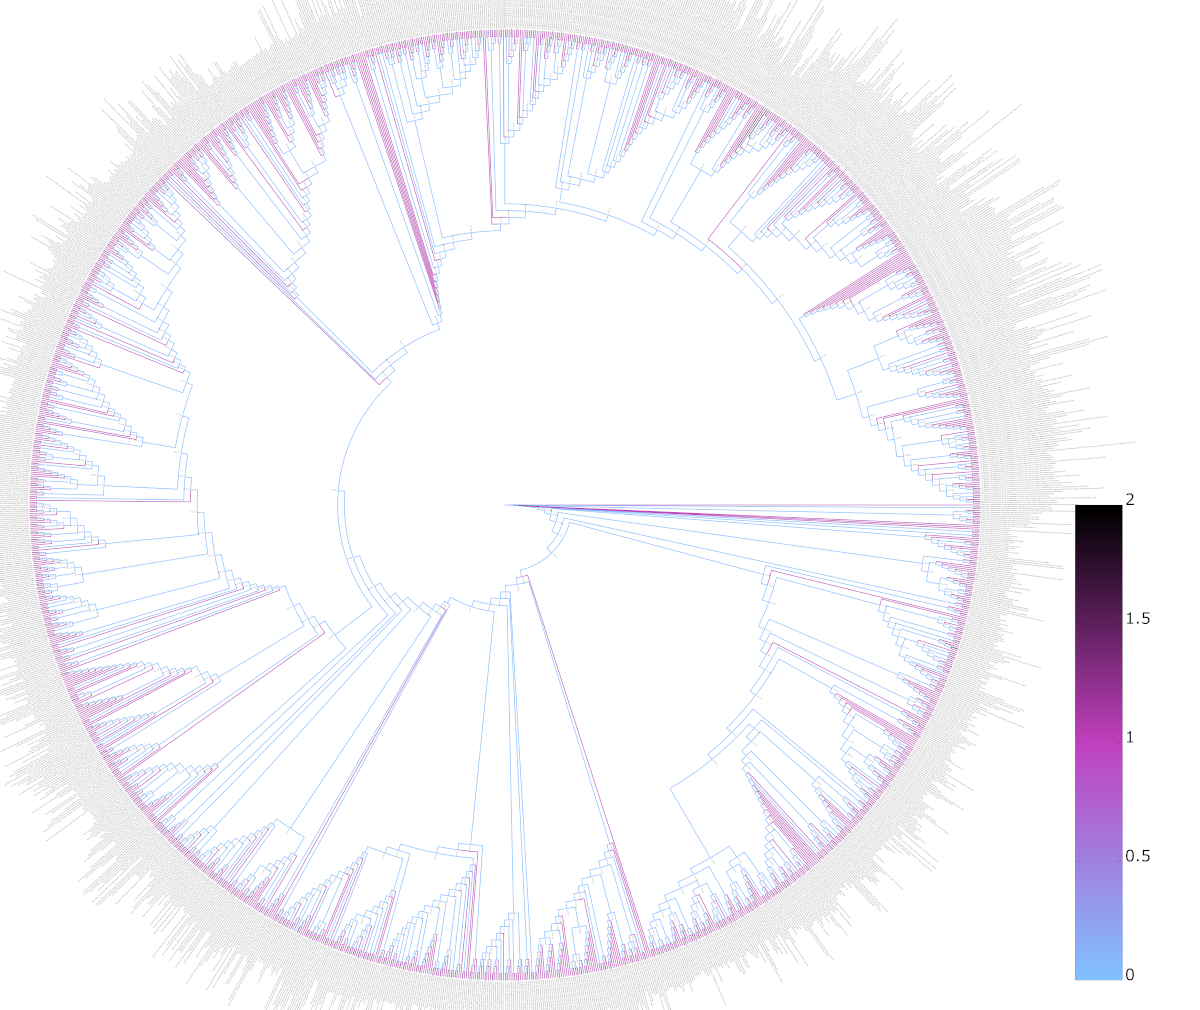
\includegraphics[width=0.65\columnwidth]{figures/darn_placemnets.png}
%    \caption{Placements of the consensus sequences used to build the COI reference phylogenetic tree for the DARN tool, onto the phylogenetic tree (stroke width for the branches of the tree is 5). The color coding represents the placements per branch, with a range from zero (blue) to a maximum of 2 (blue). The 1 leaf – 1 placement relationship, as well as the maximum of 2 placements in the color coding bar, indicate the proper placement of each consensus sequence to its corresponding branch.}
% \end{figure}


\section{A workflow for marine Genomic Observatories data analysis}






%%% Local Variables: 
%%% mode: latex
%%% TeX-master: "thesis"
%%% End: 
